%results

%What are our main findings?
%- Retail users have real impact on markets. 
%- VNs change behaviour in November already and effect markets with a 6 hour delay
%- ANVNs are as important to under market reaction

To understand the microstructure in the WSB network, we analyse the network data, described in section \ref{sec:data_desc}, with our proposed ISMB modelling approach described in section \ref{sec:method}. % using computational details as discussed in Appendix \ref{app_computation}. 
%We construct from the whole year of data hour-by-hour networks and 
%We utilize the models from Equations \eqref{eq:infl_model} and \eqref{eq:mod_fol} to model the posting behaviour of the Vital (VN) and Admissible Non-Vital Nodes (ANVN). We combine the models with the change point detection method described in Section \ref{sec:cps} 
We run ISMB with a window size of 2 months ($h =1440$ hours) and the window rolls forward with a step size of 1 week ($l = 168$ hours). %and we allow for up to $K=5$ lags. Note that the LASSO can set parameters to 0, resulting in less lags. 
To facilitate the model estimation, we set the minimum time between change points to 1 week ($k=168$).  %Window size of $h =1440$ hours (2 months), Stepsize of $l = 168$ hours (1 week), 5 Lags, and time between changepoints: $k=168$ (1 week). 
Recall that our ISMB modelling approach consists of three blocks. %In the analysis we only consider the change points which are significant based on the Vuong test. %(ie. 55 VN models out of the 64 and 41,802 ANVN models out of the 51,178).  
In section \ref{sec:resultsblock1}, we report on the modelling results of the first block focused on the determinants of users communication. In section \ref{sec:resultsblock2}, we report on the results of the second block focused on changes in behaviour. In the analysis we only consider the change points which are significant based on the Vuong test. We also report on deviance and accuracy. These results highlight the importance of ANVNs in the network evolution. In section \ref{sec:fin_analysis}, we report on the results of the third block focussed on linking the network to the market. Here we show that the individual users behaviour on Wallstreetbets influenced the market activity of the GME stock.

In addition, to get a detailed view of the network around the market frenzy, we also study the network at a 5-minute-by-5-minute frequency for the period of one month around the frenzy in section \ref{sec:5minby5min}. In section \ref{reverse_causality} we investigate for the possibility of reverse causality, meaning if the market dynamics lead to the change points instead of vice versa. Finally, in section \ref{econ_implications}, we comment on the economic and financial implications of our findings. 

%\subsection{Wallstreetbets network modeling results}
%\label{sec:hourbyhour}


%\begin{itemize}
%	\item Window size: $h =1440$ hours (2 months)
%	\item Stepsize: $l = 168$ hours (1 week)
%	\item 5 Lags
%	\item Time between changepoints: $k=168$ (1 week)
%\end{itemize}

\subsection{The determinants of users communication} \label{sec:resultsblock1}

\begin{figure}
	\caption{Value of the non-zero parameters for the VNs (left) and ANVNs (right). Darker kernels indicate more models with non-zero parameters. During trading hours (hr 14 until hr 20, UTC) there is an increases probability of posting. After comments an ANVN is likely to comment again indicated by positive $D_{out}$ and $x_{ij}$ parameters.}
	\label{fig:par-est-hour}
	\centering
	\includegraphics[scale = 0.3]{data_hour/fig_vn_parameters.png}
	\includegraphics[scale = 0.3]{data_hour/fig_nvn_parameters.png}
\end{figure}

Next, we are going to analyse the parameters of the models. As discussed in section \ref{sec:method}, we use LASSO to ensure sparsity and interpretability in the models we estimate. For the VN and ANVN models, we show the value of the non-zero parameters in Figure \ref{fig:par-est-hour}.  We observe that during trading hours the VNs have an increased probability of posting (hr 14 until hr 20). Note, we define time in UTC time zone. For the ANVNs, the effect of hours is more dispersed, which is expected as there are many more individuals. Next, we look at the dummy for trading hours ($Dum_{wls}$). Both VNs and ANVNs have predominantly positive values for this parameter, indicating that posting is more likely during market trading hours. There is a group of VNs and ANVNs that have high values (around 20) for the trading hour dummy, indicating a strong likelihood of posting during trading hours. For the VNs, the overall activity in the network seems to have no specific directional effect on the likelihood of posting, since parameter values are centered around zero. %This implies that our VN are not letting their posting behavior depend on the overall network activity. 
On the contrary, for the ANVNs the overall network activity has parameter distributions skewed to the right of the zero line, indicating a slight increase in posting likelihood of nodes, when the overall network is active. As expected, $D_{out}$ for the VNs and $D_{out,i}$ for the ANVNs is positive for the majority of the estimated parameters, indicating that when users post, they are likely to post again. However, there is also a group of users for which this parameter has a negative value around -20 to -25, indicating that these people tend to post and then probably leave the platform to come back at a later time. Finally, we consider for the VNs the effect of $X_{ii}$, which is mostly negative, indicating that after submitting a post, the VNs are less likely to submit another post. When we consider the ANVNs and the parameters of the variable $X_{ij}$, we see the opposite effect. When ANVNs submit comments to posts, they are more likely to comment again in the post. 

\begin{figure}	
	\caption{ Left: VNs $AC_{24}$, Right: ANVNs $AC_{24}$}
	\label{vital1}
	%	\centering
	\includegraphics[scale = 0.39]{data_hour/fig_vn_lik_AC24.png}
	\includegraphics[scale = 0.39]{data_hour/fig_nvn_lik_AC24.png}
\end{figure}

We observe in Figure \ref{fig:par-est-hour} that $AC^{24}$ mattered for a lot of VNs, so we compare it over time and against its relevance for the ANVNs. Figure \ref{vital1} %, \ref{vital2} 
%and \ref{vital3} 
displays for how many vital nodes the respective parameter plotted was different from $0$ over time. In Figure \ref{nonvital2}, we show various parameters which are of high importance for the ANVNs. We observe that for the VNs the activity of the network is an important variable determining their posting probability. The lagged activity $AC^{24}$ is relevant for up to $39$ vital nodes. Its relevance decreases during the market frenzy but sharply increases right after. Even though ANVNs are slightly positively impacted by network activity, only a fraction of them is impacted by it, see Figure \ref{nonvital2}. It only increases after the market frenzy. As we see from Figure \ref{fig:par-est-hour}, VNs are further impacted by their own posting behaviour and posts of others reaching them. Some of them post again once they have posted or were contacted, but also various do not post in streaks. The ANVNs show more interesting behaviour, as the bulk of parameters associated with communication are positive, compare Figure \ref{fig:par-est-hour}. 
%Figure \ref{vital3} shows that about $19\%$ of vital nodes are impacted by their in-degree $D_{in}$. However, their own past behaviour matters a lot more for their present behaviour, given the out-degree $D_{out}$ is relevant for $34\%$ of nodes and their own past threads $x_{ii}$ matter for $21\%$ of nodes. Notably, the relevance of out-degree decreases during the market frenzy, which is also the case for most variables. However, the relevance of $x_{ii}$ steadily increases with the onset of the market frenzy and continues to do so afterwards. Since the changepoints occur around the time of the market frenzy, this indicates a change in their behaviour based upon a change in impact on their behaviour as measured by the model variables. Since the relevance of network activity decreased whereas their own past activity increased in relevance, this leads to the conclusion that the vital nodes changed their behaviour from being motivated by the attention of the network towards GME to posting driven by their own behaviour. 

	\begin{figure}
	\centering
	\caption{ANVNs - Upper Left: $Din_i$, Center: $Din_i$, Right: $X_{ij}$, Lower Left: $Dout_i$, Right: $Dout_j$}
	\label{nonvital2}
	\label{nonvital3}
	\includegraphics[scale = 0.23]{data_hour/fig_nvn_lik_Din_i.png}
	\includegraphics[scale = 0.23]{data_hour/fig_nvn_lik_Din_j.png}
	\includegraphics[scale = 0.23]{data_hour/fig_nvn_lik_Xij.png} \\
	\includegraphics[scale = 0.35]{data_hour/fig_nvn_lik_Dout_i.png}
	\includegraphics[scale = 0.35]{data_hour/fig_nvn_lik_Dout_j.png}
\end{figure}

Communication initiated by the ANVNs, compare Figure \ref{nonvital2}, mattered but the communication pattern of the VN they are connected with, mattered a lot more. If the VN communicated, for $30\%$ of ANVNs, this mattered for their own posting probability. Likewise, if the VN received messages, it affected the ANVNs communication probability instantly, see Figure \ref{nonvital2}. About $33\%$ of ANVNs were affected when their VN received a message. With the onset of the market frenzy, the VNs became even more important for them, with $45\%$ of ANVNs being affected by their communication pattern. However, the most important factor was direct communication between the VN and ANVN. Before the market frenzy, it affected the communication probability of $46\%$ of ANVNs and increased with the market frenzy until it affected $64\%$ of ANVNs. This indicates a strong change in many ANVNs behaviour towards being a lot more affected by what the VNs they follow do, and also towards being impacted by posts about GME from the general network. This shows that VNs are a driving force in the network.

%\begin{figure}
%	\caption{Changepoints of vital nodes and active non-vital nodes}
%	\label{fig:cps_nvns_in_vn}
%	\centering
%	\includegraphics[scale = 0.7]{heatmap_folcp_by_infl.png}
%\end{figure}



%	\frametitle{Non-zero $AC$, $AC_{24}$ in VN models}


%	\frametitle{Receiving activity in VN models?}
%\begin{figure}
%	\caption{Vital nodes - Left: $Din$, Right: $ACthr$}
%	\label{vital2}
%	\includegraphics[scale = 0.39]{data_hour/fig_vn_lik_Din.png}
%	\includegraphics[scale = 0.39]{data_hour/fig_vn_lik_ACthr.png}
%\end{figure}


%\begin{figure}
%	\caption{Parameter Estimates ANVN. Left: hourly, Right: 5 min}
%	\label{par-est-nvn-hour}
%	\includegraphics[scale = 0.3]{data_hour/fig_nvn_parameters.png}
%	\subcaption{hourly}
%	\includegraphics[scale = 0.3]{data_5min/fig_nvn_parameters.png}
%	\subcaption{5 min}
%\end{figure}

%	\frametitle{Impact of own activity in VN models}
%\begin{figure}
%	\centering
%	\caption{Vital nodes - Left: $Din$, Center: $Dout$, Right: $X_{ii}$}
%	\label{vital3}
%	\includegraphics[scale = 0.22]{data_hour/fig_vn_lik_Din.png}
%	\includegraphics[scale = 0.22]{data_hour/fig_vn_lik_Dout.png}
%	\includegraphics[scale = 0.22]{data_hour/fig_vn_lik_Xii.png}
%\end{figure}

%\frametitle{Non-zero $AC$, $AC_{24}$ in ANVN models}

%	\frametitle{Non-zero $AC$, $AC_{24}$ in NVN models}
%	\begin{figure}
%%		\centering
%		\caption{Non-vital nodes - Left: $AC$, Right: $AC_{24}$}
%		\label{nonvital1}
%		\includegraphics[scale = 0.39]{data_hour/fig_nvn_lik_AC.png}
%		\includegraphics[scale = 0.39]{data_hour/fig_nvn_lik_AC24.png}
%	\end{figure}

%	\frametitle{How about NVNs activity? $X_{ij}$, $Dout_i$}


%	\frametitle{Impact of VN activity on NVNs activity?} %$Din_{j}$, $Dout_j$}
%\begin{figure}
%%	\centering
%	\caption{Non-vital nodes - Left: $Dout_i$, Right: $Dout_j$}
%	\label{nonvital3}
%	\includegraphics[scale = 0.39]{data_hour/fig_nvn_lik_Dout_i.png}
%	\includegraphics[scale = 0.39]{data_hour/fig_nvn_lik_Dout_j.png}
%\end{figure}



%\begin{figure}
%	\includegraphics[scale = 0.5]{changepoint_search.jpg}
%\end{figure}
%\subsection{Change points identified}
%

%To sum up, we find that the VNs and ANVN show change in their posting behavior during the year and that these changepoints can be related to external events. In addition, the parameters of the model give us insight into the determinants for posting behavior and show that VNs affect the posting probability of ANVN. 

\subsection{The importance of admissible non-vital nodes} \label{sec:resultsblock2}

\begin{table} 
	\caption{Number of identified change points after applying our proposed ISMB modelling approach to the WSB network. We find that the majority of the VNs and ANVNs change their posting behaviour once.}
	\label{tab:changepoints}
	\centering
	\begin{tabular}[t]{lrrrr}
		\hline \hline
		No. cps&VN&\% & ANVN &\%\\
		\hline \hline
		0&13&20.3&14339&28.02\\
		1&50&78.1&36618&71.55\\
		2&1&1.6&210&0.41\\
		3&0&0.0&11&0.02\\
		$\geq 4$&0&0.0&0&0.00\\
		\hline \hline
	\end{tabular}
\end{table}
Next we study the change point results of ISMB. These change points identify the changes in users believes which in the theory of \citet{Pedersen2022} is the link between the social network and the markets. First, we analyse the identified change points in our models, reported in Table \ref{tab:changepoints}. Note that these change points are statistically significant at a 5\% level as tested with the Vuong test. We see that most VNs and ANVNs change their posting behaviour once in the year (78\% and 72\%) whereas 20\% of the VN and 28\% of the ANVN do not have any change points in their models. The maximum number of change points we find is 3. 
Figure \ref{fig:cp_over_time} shows the change points of all VN (left) and all ANVN (right) over time. We see that some VNs change their behaviour as early as November and December 2020 which is well before the frenzy. On the contrary, most ANVNs change their behaviour during and after the frenzy. In Figure \ref{fig:cps_frenzy}, we zoom in on the period around the frenzy and look at the ANVNs' change points. There are large peaks at specific moments in time, which indicate hours during which many ANVNs (up to 2000) show change in their posting behaviour. Figure \ref{fig:cps_frenzy} also indicates key events (taken from \cite{GMETimeline}) and the posts of Keith Gill. We see that various events, but not all, coincide in time with large peaks in the number of change points we find for the ANVN models. Whereas studies such as \textcite{Gan2020} highlight the relevance of overall network activity and \textcite{Yang2015} show influential nodes like the VN are most important, this highlights the importance of monitoring individual and less important users change in behaviour. It also shows that monitoring news instead of the network would have missed or overestimated the relevance of events, given users reacted strongly to some and others only slightly. 
Occurring in bulk and even when controlling for network activity, they lead to market reactions as we show in section \ref{sec:fin_analysis}. 

\begin{figure}
	\caption{Identified significant change points over time for VN (left) and ANVN (right). Some VNs change their behaviour as early as November 2020 which is well before the frenzy. On the contrary, most ANVNs change their behaviour during and after the frenzy.}
	\label{fig:cp_over_time}
	\centering
	\includegraphics[scale = 0.3]{data_hour/cps_over_time_VN.png}
	\includegraphics[scale = 0.3]{data_hour/cps_over_time_NVN.png}
\end{figure}


\begin{figure}
	\caption{Change points over time for ANVNs during frenzy period labelled with external events}
	\label{fig:cps_frenzy}
	\centering
	\includegraphics[scale = 0.4]{data_hour/cps_over_time_NVN_frenzy.png}
\end{figure}


%To study the identified changepoints in more detail we look at each Vital Node in Figure \ref{fig:cps_nvns_in_vn}. The dots indicate a changepoint of a vital node and we place it in relation to the changepoints of active non-vital nodes which comment in the post of the respective vital nodes. We observe that most of the changepoints which define the behaviour of the nodes takes place right when the market frenzy starts. A few of them even change their behaviour up to 2 months before that. Further changepoints appear a few weeks after the frenzy which would be in line with the rational that after the frenzy ebbed off, users would change their posting behaviour. We observe a particularly large amount of changepoints of ANVNs who comment in the post of a particular VN, 4300. This user is Keith Gill, which shows that his posts indeed triggered changes of users behaviour. The change of users behaviour is the most intense right before and during the market frenzy, which raised the question what exactly triggered the users change in behaviour. Another user also triggered the change of many users behaviour however mostly during and after the market frenzy. This is the founder of Wallstreetbets who regularly submits posts asking users opinions about particular stocks and their plans for investments in the week following. 
To study in more detail the reaction of ANVNs to VNs change points, we look at the time between the VNs (first) change point and the ANVNs (first) change point. Figure \ref{fig:time_between_cps} shows a density plot of these times for the most active vital nodes 4300 and 1583 as well as all the other VNs. We see that especially for VN 4300, the change in posting behaviour seems to result in ANVNs changing their posting behaviour a while later, with the peak of the distribution at 400 hours (16 days) after VN 4300 changed its behaviour. For VN 1583, a well-known moderator on WSB, the effect is less pronounced and inline with the role of moderators \citep{he2024platform} which are more reactive to the network. Again, this indicates that only looking at important nodes such as VNs does not suffice. 


\begin{figure}
	\caption{Time between change points of VNs and change points of ANVNs.}
	\label{fig:time_between_cps}
	\centering
	\includegraphics[scale = 0.5]{data_hour_folcp_by_infl_allignedatzero.png}
\end{figure}

We evaluate model deviance and accuracy to understand how well our model fits and predicts the users posting behaviour and how important it is to include change points in our modelling approach. Figure \ref{fig:deviance} shows the percentage decrease in deviance where we compare our model to a model with intercept-only and without change points. By this, we investigate if the variables and change point detection method we suggest, improves the prediction of users communication behaviour. We see that our model decreases the deviance substantially. Figure \ref{fig:accuracy} shows the percentage points increase in prediction accuracy of our model compared to the intercept model without change points. We only consider the predictions of communications (ie. the $1$'s in our data) as the data is highly unbalanced. For the VNs, we see a small group of models for which we predict all communications accurately and overall the accuracy is better for the models with change points than the base line model without change points. This shows the outperformance of our modelling framework for modelling and analysing individual users posting behaviour. 
%\footnote{ modify the selection of significance now we use significant model if any of our three tests (lik, bic, aic) are smaller than 5 percent. Might want to make a choice. }
\begin{figure}
	\caption{Relative decrease in deviance for our model compared to an intercept model without change points. Left: VNs, Right: ANVNs}
	\label{fig:deviance}
	\centering
	\includegraphics[scale = 0.3]{data_hour/Deviance_histo_VN.png}
	\includegraphics[scale = 0.3]{data_hour/Deviance_histo_NVN.png}
\end{figure}

\begin{figure}
	\caption{Percent points increase in prediction accuracy for our model compared to an intercept model without change points. Left: VNs, Right: ANVNs}
	\label{fig:accuracy}
	\centering
	\includegraphics[scale = 0.3]{data_hour/Accuracy_histo_VN.png}
	\includegraphics[scale = 0.3]{data_hour/Accuracy_histo_NVN.png}
\end{figure}


\subsection{Impact of Wallstreetbets on GME stock price}
\label{sec:fin_analysis}
In this subsection, we link the user behavior to the financial markets and study the affect on the return and volatility of the GME stock. We first perform a full sample analysis on an hour-by-hour basis followed by a detailed study of the frenzy period on a 5minute-by-5minute basis.


\subsubsection{Hourly analysis: Changes in users behaviour and market impact}
%%%%%
% now a summary of the full scale analysis with focus on significant parameters only
%%%%%
%\input{Returnmodels1_t.tex}

% Table created by stargazer v.5.2.3 by Marek Hlavac, Social Policy Institute. E-mail: marek.hlavac at gmail.com
% Date and time: Tue, Feb 06, 2024 - 18:15:42
\begin{table}[!htbp] \centering 
  \caption{Modeling returns with equation \eqref{eq:ret}. Columns show different combinations of included features. For the sake of brevity insignificant variables and significant lagged return variables are not displayed. } 
  \label{Returnmodels1_t} 
\tiny 
\begin{tabular}{@{\extracolsep{5pt}}lcccccc} 
\\[-1.8ex]\hline 
\hline \\[-1.8ex] 
 & \multicolumn{6}{c}{\textit{Dependent variable: return}} \\ 
\cline{2-7} 
\\[-1.8ex] & (1) & (2) & (3) & (4) & (5) & (6)\\ 
\hline \\[-1.8ex] 
 %ret lagged & Yes & Yes & Yes & Yes & Yes & Yes \\  \hline
& & & & & & \\
 VN3 &  &  & $-$0.021$^{***}$ & $-$0.020$^{***}$ &  & $-$0.022$^{***}$ \\ 
 &  &  & (0.007) & (0.006) &  & (0.006) \\ 
 & & & & & & \\ 
 VN4 &  &  & 0.006 & 0.012$^{**}$ &  & 0.008 \\ 
 &  &  & (0.006) & (0.006) &  & (0.006) \\ 
 & & & & & & \\ 
 NVN &  &  &  & $-$0.004$^{***}$ &  & $-$0.003$^{***}$ \\ 
 &  &  &  & (0.001) &  & (0.001) \\ 
 & & & & & & \\ 
 NVN1 &  &  &  & 0.007$^{***}$ &  & 0.008$^{***}$ \\ 
 &  &  &  & (0.001) &  & (0.001) \\ 
 & & & & & & \\ 
 NVN2 &  &  &  & 0.002$^{**}$ &  & 0.003$^{***}$ \\ 
 &  &  &  & (0.001) &  & (0.001) \\ 
 & & & & & & \\ 
 NVN3 &  &  &  & $-$0.004$^{***}$ &  & $-$0.004$^{***}$ \\ 
 &  &  &  & (0.001) &  & (0.001) \\ 
 & & & & & & \\ 
 NVN6 &  &  &  & $-$0.001$^{*}$ &  & $-$0.001$^{*}$ \\ 
 &  &  &  & (0.001) &  & (0.001) \\ 
 & & & & & & \\ 
 Constant & 0.0003 & 0.0002 & 0.0002 & 0.001 & 0.0003 & 0.001 \\ 
 & (0.0004) & (0.001) & (0.001) & (0.001) & (0.001) & (0.001) \\ 
  & & & & & & \\ 
\hline \\[-1.8ex] 
Lagged returns & Yes & Yes & Yes & Yes & Yes & Yes \\ 
Vital nodes & No & No & Yes & Yes & No & Yes \\ 
Non-vital nodes & No & No & No & Yes & No & Yes \\ 
Network activity & No & Yes & Yes & Yes & Yes & Yes \\ 
Network statistics & No & No & No & No & Yes & Yes \\ 
\hline &  &  &  &  &  &  \\ 
Observations & 1,633 & 1,633 & 1,633 & 1,633 & 1,633 & 1,633 \\ 
R$^{2}$ & 0.009 & 0.020 & 0.028 & 0.081 & 0.045 & 0.124 \\ 
Adjusted R$^{2}$ & 0.004 & 0.011 & 0.014 & 0.064 & 0.021 & 0.093 \\ 
\hline 
\hline \\[-1.8ex] 
\textit{Note:}  & \multicolumn{6}{r}{$^{*}$p$<$0.1; $^{**}$p$<$0.05; $^{***}$p$<$0.01} \\ 
\end{tabular} 
\end{table} 


We conduct a full sample analysis, which allows us to analyse the parameters driving the stock dynamic. 
We observe for the VNs and ANVNs a significant effect on the return, integrated variance (IV) and jump volatility (JV) of GME, compare Tables \ref{Returnmodels1_t}, \ref{IVmodels1_t}, and \ref{Jmodels1_t}. \str{We observe only little effect onto trading volume (TV), see Table XXX. It is well documented that users of WSB primarily traded options, for which we observe a stronger predictability, see Table XXX. However, the improvement is not as strong as for return, IV, and JV.} When adding the $VN$ change points, a significant parameter occurs in lag $6$ for IV and JV. This infers that it takes 6 hours until the change in behaviour of VNs is reflected in the integrated variance and jump volatility of the GME stock. This is reasonable given the change in behaviour will be accompanied by a post on WSB and it would take a while until sufficient users have seen the post, reacted to it and (potentially) acted based on it on the stock market. For the return, we observe a faster effect from the VNs, materialising already after 3 hours. As for the $ANVNs$, we see an even more drastic increase in the adjusted $R^2$, and various variables over several lags are significant. Notably, the market reacts faster to their changes in behaviour. We observe this from earlier lags being significant. Given the different roles of VNs and ANVNs in the network, it is reasonable that the effect of ANVNs is reflected faster in the market. %Given there are a lot more users in the group of the ANVNs as the VN, a lot of change points occurred around the same time and reflected a change of various users behaviour. Hence it is reasonable that this effect is faster reflected. Again, the effect materialises faster for the return compared to the IV and JV. 
\str{Whereas the effects of the change points of VNs and ANVNs on predictability is pronounced for return, IV, and JV, the same is not true for trading volume and option trading volume. The users of WSB are known for trading options instead of on spot markets, hence it is unsurprising that the effect upon trading volume is minor, see Table XXX. The predictability of option trading volume is generally higher, see Table XXX, but including change points of VNs and ANVNs does not improve the adj. $R^2$. These results show that the volume users traded was not affected by users change in behaviour, suggesting that the change in behaviour did not bring in additional trading activity, while affecting returns and volatility (IV, JV) though.} 
\str{All models containing VNs and ANVNs change points as variables, also contain the network activity as a variable. In light of this, it is worth pointing out that the network activity $AC$ does not proxy the individual users change in behaviour, but remains statistically significant for the market predictability. This shows that the change points measure user behaviour the overall network activity cannot represent. Further, it is not only the majority over users who matter, but also the influential users, since the change in behaviour from VNs remains important for the explainability of the return, integrated variance\str{, jump volatility, and trading volume}}. %As for the trading volume, for which we observed only little explainability from change points of the VN and ANVN in the rolling window analysis, we still record explainability from time lagged change points of the VNs and ANVNs. Whereas the low explainability of the TV is surprising at first, this may be due to the trading of GME having taken place largely via derivatives. Their trading volume is not reflected in the TV of the spot market. 

%\input{IVmodels1_t.tex}

% Table created by stargazer v.5.2.3 by Marek Hlavac, Social Policy Institute. E-mail: marek.hlavac at gmail.com
% Date and time: Wed, Mar 01, 2023 - 17:05:28
\begin{table}[!htbp] \centering 
 \caption{Modeling integrated variance (IV) with equation \eqref{eq:ret}. Columns show different combinations of included features. For the sake of brevity insignificant variables and significant lagged IV variables are not displayed. } 
  \label{IVmodels1_t} 
\tiny 
\begin{tabular}{@{\extracolsep{5pt}}lcccccc} 
\\[-1.8ex]\hline 
\hline \\[-1.8ex] 
 & \multicolumn{6}{c}{\textit{Dependent variable: integrated variance (IV)}} \\ 
\cline{2-7} 
\\[-1.8ex] & (1) & (2) & (3) & (4) & (5) & (6)\\ 
\hline \\[-1.8ex] 
 %IV lagged & Yes & Yes & Yes & Yes & Yes & Yes \\ \hline
& & & & & & \\ 
 VN6 &  &  & 0.064$^{***}$ & 0.065$^{***}$ &  & 0.061$^{***}$ \\ 
 &  &  & (0.006) & (0.006) &  & (0.006) \\ 
 & & & & & & \\ 
 NVN &  &  &  & $-$0.003$^{***}$ &  & $-$0.004$^{***}$ \\ 
 &  &  &  & (0.001) &  & (0.001) \\ 
 & & & & & & \\ 
 NVN1 &  &  &  & 0.005$^{***}$ &  & 0.004$^{***}$ \\ 
 &  &  &  & (0.001) &  & (0.001) \\ 
 & & & & & & \\ 
 NVN2 &  &  &  & 0.001 &  & 0.002$^{**}$ \\ 
 &  &  &  & (0.001) &  & (0.001) \\ 
 & & & & & & \\ 
 NVN3 &  &  &  & 0.002$^{*}$ &  & 0.003$^{***}$ \\ 
 &  &  &  & (0.001) &  & (0.001) \\ 
 & & & & & & \\ 
 NVN4 &  &  &  & $-$0.002$^{**}$ &  & $-$0.002$^{*}$ \\ 
 &  &  &  & (0.001) &  & (0.001) \\ 
 & & & & & & \\ 
 NVN5 &  &  &  & $-$0.003$^{***}$ &  & $-$0.003$^{***}$ \\ 
 &  &  &  & (0.001) &  & (0.001) \\ 
 & & & & & & \\ 
 Constant & 0.001$^{***}$ & $-$0.002$^{**}$ & $-$0.001$^{**}$ & $-$0.001$^{*}$ & $-$0.0004 & $-$0.0004 \\ 
 & (0.0004) & (0.001) & (0.001) & (0.001) & (0.001) & (0.001) \\ 
 & & & & & & \\ 
 \hline \\[-1.8ex] 
 Lagged IV & Yes & Yes & Yes & Yes & Yes & Yes \\ 
 Vital nodes & No & No & Yes & Yes & No & Yes \\ 
 Non-vital nodes & No & No & No & Yes & No & Yes \\ 
 Network activity & No & Yes & Yes & Yes & Yes & Yes \\ 
 Network statistics & No & No & No & No & Yes & Yes \\ 
 \hline &  &  &  &  &  &  \\ 
 Observations & 1,633 & 1,633 & 1,633 & 1,633 & 1,633 & 1,633 \\ 
 R$^{2}$ & 0.175 & 0.189 & 0.239 & 0.265 & 0.255 & 0.328 \\ 
 Adjusted R$^{2}$ & 0.172 & 0.182 & 0.228 & 0.250 & 0.237 & 0.304 \\ 
\hline 
\hline \\[-1.8ex] 
\textit{Note:}  & \multicolumn{6}{r}{$^{*}$p$<$0.1; $^{**}$p$<$0.05; $^{***}$p$<$0.01} \\ 
\end{tabular} 
\end{table} 

%\input{IVmodels2_t.tex}


%\input{Jmodels1_t.tex}

% Table created by stargazer v.5.2.3 by Marek Hlavac, Social Policy Institute. E-mail: marek.hlavac at gmail.com
% Date and time: Wed, Mar 01, 2023 - 17:05:31
\begin{table}[!htbp] \centering 
  \caption{Modeling integrated variance (IV) with equation \eqref{eq:ret}. Columns show different combinations of included features. For the sake of brevity insignificant variables are not displayed. } 
  \label{Jmodels1_t} 
\tiny 
\begin{tabular}{@{\extracolsep{5pt}}lccccc} 
\\[-1.8ex]\hline 
\hline \\[-1.8ex] 
 & \multicolumn{5}{c}{\textit{Dependent variable: Jump volatility (JV)}} \\ 
\cline{2-6} 
\\[-1.8ex] & (1) & (2) & (3) & (4) & (5)\\ 
\hline \\[-1.8ex] 
 VN6 &  & $-$0.028$^{***}$ & $-$0.028$^{***}$ &  & $-$0.028$^{***}$ \\ 
 &  & (0.007) & (0.008) &  & (0.007) \\ 
 & & & & & \\ 
 NVN &  &  & $-$0.003$^{**}$ &  & $-$0.003$^{**}$ \\ 
 &  &  & (0.001) &  & (0.001) \\ 
 & & & & & \\ 
 NVN1 &  &  & 0.006$^{***}$ &  & 0.006$^{***}$ \\ 
 &  &  & (0.001) &  & (0.001) \\ 
 & & & & & \\ 
 NVN3 &  &  & $-$0.002$^{**}$ &  & $-$0.002 \\ 
 &  &  & (0.001) &  & (0.001) \\ 
 & & & & & \\ 
 NVN5 &  &  & 0.002$^{**}$ &  & 0.002$^{**}$ \\ 
 &  &  & (0.001) &  & (0.001) \\ 
 & & & & & \\ 
 Constant & $-$0.001 & $-$0.001$^{*}$ & $-$0.001 & $-$0.002$^{**}$ & $-$0.002$^{*}$ \\ 
 & (0.001) & (0.001) & (0.001) & (0.001) & (0.001) \\ 
 & & & & & \\ 
 \hline \\[-1.8ex] 
 Vital nodes & No & Yes & Yes & No & Yes \\ 
 Non-vital nodes & No & No & Yes & No & Yes \\ 
 Network activity & Yes & Yes & Yes & Yes & Yes \\ 
 Network statistics & No & No & No & Yes & Yes \\ 
 \hline &  &  &  &  &  \\ 
 Observations & 1,633 & 1,633 & 1,633 & 1,633 & 1,633 \\ 
 R$^{2}$ & 0.022 & 0.032 & 0.045 & 0.102 & 0.130 \\ 
 Adjusted R$^{2}$ & 0.017 & 0.022 & 0.031 & 0.084 & 0.103 \\ 
\hline 
\hline \\[-1.8ex] 
\textit{Note:}  & \multicolumn{5}{r}{$^{*}$p$<$0.1; $^{**}$p$<$0.05; $^{***}$p$<$0.01} \\ 
\end{tabular} 
\end{table} 

%\input{Jmodels2_t.tex}

%\input{Volumemodels1_t.tex}

% Table created by stargazer v.5.2.3 by Marek Hlavac, Social Policy Institute. E-mail: marek.hlavac at gmail.com
% Date and time: Thu, Oct 15, 2026 - 12:31:48
\begin{table}[!htbp] \centering 
  \caption{Significant variables from models 13 with differing variables include 
                               and Lag length 7. Insignificant variables are not displayed. 
                               Control variables (network statistics and network activity) are 
                               included for differing models.} 
  \label{Volumemodels1_t} 
\scriptsize 
\begin{tabular}{@{\extracolsep{5pt}}lcccccc} 
\\[-1.8ex]\hline 
\hline \\[-1.8ex] 
 & \multicolumn{6}{c}{\textit{Dependent variable: Trading Volume (TV)}} \\ 
\cline{2-7} 
\\[-1.8ex] & (1) & (2) & (3) & (4) & (5) & (6)\\ 
\hline \\[-1.8ex] 
 VN2 &  &  & 1.762$^{***}$ & 1.798$^{***}$ &  & 1.784$^{***}$ \\ 
  &  &  & (0.350) & (0.352) &  & (0.355) \\ 
  & & & & & & \\ 
 Constant & 0.046$^{**}$ & 0.057 & 0.057$^{*}$ & 0.051 & 0.057 & 0.058 \\ 
  & (0.020) & (0.035) & (0.035) & (0.037) & (0.042) & (0.042) \\ 
  & & & & & & \\ 
\hline \\[-1.8ex] 
Lagged TV & Yes & Yes & Yes & Yes & Yes & Yes \\ 
Vital nodes & No & No & Yes & Yes & No & Yes \\ 
Non-vital nodes & No & No & No & Yes & No & Yes \\ 
Network activity & No & Yes & Yes & Yes & Yes & Yes \\ 
Network statistics & No & No & No & No & Yes & Yes \\ 
\hline &  &  &  &  &  &  \\ 
Observations & 1,633 & 1,633 & 1,633 & 1,633 & 1,633 & 1,633 \\ 
R$^{2}$ & 0.012 & 0.014 & 0.031 & 0.034 & 0.026 & 0.047 \\ 
Adjusted R$^{2}$ & 0.007 & 0.005 & 0.017 & 0.016 & 0.002 & 0.014 \\ 
\hline 
\hline \\[-1.8ex] 
\textit{Note:}  & \multicolumn{6}{r}{$^{*}$p$<$0.1; $^{**}$p$<$0.05; $^{***}$p$<$0.01} \\ 
\end{tabular} 
\end{table} 


%\input{opt_Volumemodels1_t.tex}

% Table created by stargazer v.5.2.3 by Marek Hlavac, Social Policy Institute. E-mail: marek.hlavac at gmail.com
% Date and time: Thu, Oct 15, 2026 - 12:32:02
\begin{table}[!htbp] \centering 
  \caption{Significant variables from models 13 with differing variables include 
                               and Lag length 7. Insignificant variables are not displayed. 
                               Control variables (network statistics and network activity) are 
                               included for differing models.} 
  \label{opt_Volumemodels1_t} 
\scriptsize 
\begin{tabular}{@{\extracolsep{5pt}}lcccccc} 
\\[-1.8ex]\hline 
\hline \\[-1.8ex] 
 & \multicolumn{6}{c}{\textit{Dependent variable: Option Trading Volume (OTV)}} \\ 
\cline{2-7} 
\\[-1.8ex] & (1) & (2) & (3) & (4) & (5) & (6)\\ 
\hline \\[-1.8ex] 
 NVN &  &  &  & $-$0.061$^{*}$ &  & $-$0.070$^{*}$ \\ 
  &  &  &  & (0.036) &  & (0.036) \\ 
  & & & & & & \\ 
 Constant & $-$0.001 & $-$0.054 & $-$0.055 & $-$0.072$^{**}$ & $-$0.079$^{**}$ & $-$0.095$^{**}$ \\ 
  & (0.020) & (0.034) & (0.034) & (0.036) & (0.039) & (0.040) \\ 
  & & & & & & \\ 
\hline \\[-1.8ex] 
Lagged Option TV & Yes & Yes & Yes & Yes & Yes & Yes \\ 
Vital nodes & No & No & Yes & Yes & No & Yes \\ 
Non-vital nodes & No & No & No & Yes & No & Yes \\ 
Network activity & No & Yes & Yes & Yes & Yes & Yes \\ 
Network statistics & No & No & No & No & Yes & Yes \\ 
\hline &  &  &  &  &  &  \\ 
Observations & 1,687 & 1,687 & 1,687 & 1,687 & 1,687 & 1,687 \\ 
R$^{2}$ & 0.209 & 0.215 & 0.217 & 0.221 & 0.233 & 0.240 \\ 
Adjusted R$^{2}$ & 0.205 & 0.208 & 0.206 & 0.206 & 0.215 & 0.214 \\ 
\hline 
\hline \\[-1.8ex] 
\textit{Note:}  & \multicolumn{6}{r}{$^{*}$p$<$0.1; $^{**}$p$<$0.05; $^{***}$p$<$0.01} \\ 
\end{tabular} 
\end{table} 


The explainability of the returns is remarkably high when considering the users change points in the model. Commonly asset returns experience a lot lower $R^2$. To explore the dynamics over time further, we conduct a rolling window analysis. We apply model \eqref{eq:ret} %, (\ref{eq:IV}), (\ref{eq:JV}), and (\ref{eq:vol}) 
during the rolling window analysis on 3 months of data and roll forward with step width of 1 hour. Figure \ref{fig:rolling_return} %, \ref{fig:rolling_iv}, \ref{fig:rolling_jv}, and \ref{fig:rolling_tv} 
summarises the adjusted $R^2$ on the rolling windows of 4 different model specifications, each containing a different subset of the variables of interest. The black line contains the benchmark model consisting of the time series own past (7 lags of returns) %, past integrated volatility, past trading volume respectively) 
and aggregated network activity (AC), contemporaneous and also with 7 lags, as explainable variables. This number of lags were chosen as they span the past trading day, i.e. if we model the return at 11 am, 11.01.21, then 7 lags span back until 11 am, 10.01.21, since we only consider market opening hours. The red line adds the VN change points to the model and the green one the ANVN change points. To compare if the change points of the VN and ANVNs contain additional information, which cannot be captured by regular network statistics (log mean distance, log mean degree, log number of active nodes), the blue line shows the adjusted $R^2$ of the model containing AC and the network statistics. 

We observe from Figure \ref{fig:rolling_return}, that the change points of the VN and ANVN add to the explainability of the GME return dynamics. Before the market frenzy, from August to December, the model containing AC, VN and ANVN change points (green), results in much higher adjusted $R^2$, up to $0.12$. For return predictability, this is already remarkably high. This suggests that the VN and ANVNs were already a decisive force for the price dynamics. Note that the model containing the returns own past and AC, as well as the network statistics additionally, result in much lower adjusted $R^2$, between $0-0.05$. Interestingly, the adjusted $R^2$ drops strongly for all models in December, during the building up period of the frenzy. This may suggest that during this brief period, the former notable explainability from VN and ANVNs change in behaviour was priced into GMEs stock price. During the market frenzy itself, the return explainability reaches remarkably high adjusted $R^2$ of up to \str{$0.28$}. The return predictability from the users' changes in behaviour remains very high during the entirety of the market frenzy, showing the impact the social network had on the market during that time. It is further remarkable, that classical network measures such as AC and the network statistics were not able to explain the market movements that well. The explainability of the return dynamics from the changes of users behaviour remained high also after the frenzy, outperforming all other models, showing that the social network had a longer lasting effect on the markets, going beyond the main market frenzy. 

\begin{figure}
	\caption{Adj. $R^2$ for return models with rolling window over 3 months with step width 1 hour. Change points of the VN and ANVN add to the explainability of the GME return dynamics.}
	\label{fig:rolling_return}
	\centering
	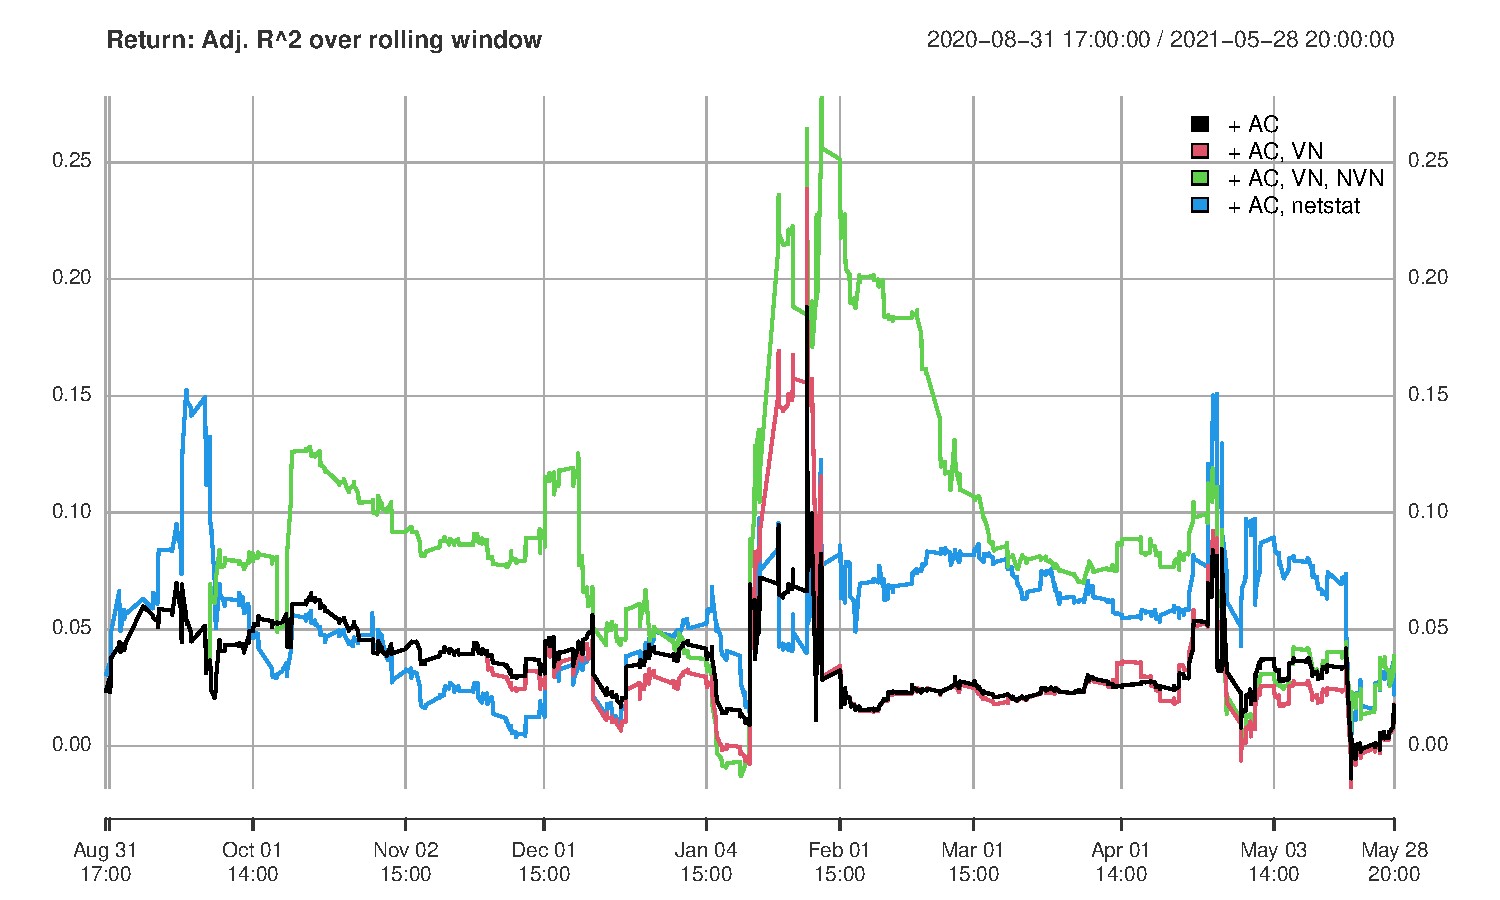
\includegraphics[scale = 0.5]{adjR2_return_rolling.pdf}
\end{figure}


%\input{Volumemodels1_t.tex}

%Turning towards integrated and jump volatility, an interesting pattern emerges, compare Figures \ref{fig:rolling_iv} and \ref{fig:rolling_jv}. Note that the models are similar to the return one, but that the jump volatility model does not contain past jumps as explainable variable as jumps are independent and random by definition. For integrated variance, we observe that the change points of VN and ANVN excel in explaining its dynamic with the onset of the market frenzy. After the frenzy, the explainability from the changes in users behaviour remain high and excel in explaining its dynamics compared to all other model specifications. Even values of up to $0.7$ in adjusted $R^2$ are observed following the market frenzy whereas the next best model only reaches $0.4$. This infers that the role the social network played in the market frenzy, in particular individual users change in behaviour, caused a longer running change in the drivers of integrated variance. 

%For jump volatility, Figure \ref{fig:rolling_jv}, we observe a remarkably high explainability from the users' change in behaviour. Already months before the actual market frenzy, the users change in behaviour explained for a while $80\%$ of the jump dynamics (adj. $R^2$), before dropping to a range of $20-40\%$. Note that leaving out the changepoints as explainable variables from the model resulted in tremendously lower explainability of the jump dynamics, consistently way below the VN and ANVN changepoint model. Note that no model was able to explain the jump dynamics during December, but with the onset of the market frenzy, again the changes in users behaviour strongly improved the explainability of the occurrence of jumps in volatility. Towards the mid of the year, months after the market frenzy took place, explainability of users change in behaviour increased again and outperformed other specifications. 
%For trading volume, Figure \ref{fig:rolling_tv}, we observe a mixed picture. Overall the adjusted $R^2$ is low for all model specifications, but the change in users behaviour hardly ever explains the trading volume dynamics better than other variables. Only during the period of the direct aftermath of the market frenzy, the changes in users' behaviour improve the trading volume explainability. 

In summary, these results show that the changes in users behaviour have a strong and long lasting effect on the return dynamics. In particular, changes in ANVN-users behaviour excel in doing so, VN-users play a lesser role in explaining the return dynamics. This implies that not only highly influential users, despite inciting communication in the network, had an effect on the market. Their impact is comparably less pronounced than the changes in behaviour emerging from the masses of users on the social network. 

%We also investigate if the detection of the changepoints and their explainability for the dynamics of the integrated variance could be proxied by the network measures mean distance, mean degree and number of active nodes. These measures proxy network activity and importance of nodes. However, including them instead of the $VN$ and $NVN$ changepoints, yields a tremendously lower $R^2$ of $0.255$ compared to $0.392$ when $VN$ and $NVN$ are included but the network control statistics are not. 
%
%As we established, the changepoints have a strong and significant impact on the integrated variance. On the jump component, $JV$, which is by its nature a short-lived part of the variance, the change in behaviour of users has less of an impact, compare Table \ref{Jmodels1_t}. The $R^2$ increases strongly with the exponential weighting specifications for the changes behaviour, (\ref{eq:spec2}), however the impact is not as strong as for the network statistics. Given this is the jump component of the variance, this infers that the change in users behaviour is not strongly related to the immediate excesses in the GME variance. However it is strongly related to the integrated part of the variance, hence the regular variance. 
%
%We further investigate if not only the variance of GME is explained by the behaviour of users on WSB, but also if the return of GME is determined by it. We observe a persistent increase in terms of $R^2$ and also adjusted $R^2$ when adding network activity and the vital nodes changepoints, VN, to the model comprised of the hourly lagged return of GME, compare Table \textcolor{red}{TABLE HAS NO LABEL YET}. The largest increase takes place when the changepoints of the Non-Vital Nodes, ANVN, is being added to the model. We observe a $R^2$ and adjusted $R^2$ of 0.132 and 0.115 respectively. We observe that all ANVN variables, the contemporaneous and lagged ones, are significant and in combination with the drastically increasing model fit, we conclude that the changepoints of the Non-Vital Nodes has high explainability for the GME return evolution. The model containing only the network statistics does not reach achieve an equally high $R^2$, consequently the VN and ANVN indeed explain the return movements of GME better than established network statistics. Adding said network statistics to the model containing also the VN and ANVN, achieves an even higher $R^2$ and adjusted $R^2$, which suggests that the VN and ANVN explain part of the return movements which are not captured by the network statistics, network activity and also not by the past return movements. 
%
%Likewise we investigate if the dynamics of the trading volume (TV) of GME is explained by the changepoints of the Vital Nodes (VN) and Non-Vital Nodes (NVN). We observe that the variables embedded in model (\ref{eq:vol}) explain parts of the dynamics of the trading volume. The $R^2$ and adjusted $R^2$ reach the best values for the model containing the past trading volume, network activity and VN. Note that the VN parameter is significant whereas none of the AC parameters is significant. We observe that adding the ANVN and network statistics causes a decrease in the adjusted $R^2$, conseqeuntly including them only marginally increases the explainability of the system. As in the previous examinations, we conclude that the changepoints of the vital nodes, VN, explain the dynamics of the trading volume. 

%The baseline model we compare against contains the parameters $r_{t-1}$ and $AC_{t}$ for the contemporaneous model and $r_{t-1}$ and $AC_{t-1}$ for the time lagged model. This specification follows the markov property that past returns predict future ones and that the activity of a network impacts related stock returns. We observe that for the contemporaneous model, the parameter $AC_{t}$ is significant and the $R^2$ is $0.016$. When adding $cp_{vn;t}$ and $cp_{nvn;t}$ to the model, the network variable parameter becomes insignificant while the $R^2$ increases as well as the adjusted $R^2$, Table \ref{table_return_contem}. Simultaneously $cp_{vn;t}$ is significant which suggests that the actual reason for the observation that the network activity impacts the return of GME, the actual reason for this was the change in behaviour of vital nodes on the Wallstreetbets network. Given that alternative measures for a networks state such as mean degree, distance and active nodes exist, we add these variables to the model which increases the $R^2$. Notably the vital nodel changepoint variable remains significant. 

%Considering that changes in ones behaviour are not an isolated event but rather an event with a potentially lasting effect for a while, we analyse if $cp_{vn,ews;t}$ and $cp_{nvn,ews;t}$ impacts the return. We set $\lambda = 0.8$. Again, the changepoints of the vital nodes are significant and also the ones for the non-vital nodes become significant. Notably the $R^2$ increases as does the adjusted $R^2$. 

%After having established that the contemporaneous effect of the changepoints impacts the market return of GME, we investigate the time lagged effect, Table \ref{table_return_timelagged}. The results remain similar which shows that also past changepoints of vital and non-vital nodes impacts the returns of GME. Notably the $R^2$ decreases compared to the contemporaneous model however the significance of the parameters remains. 

%In a similar setup as for the return, we are analysing if the Wallstreetbets network and the changepoints of the nodes impact the realized volatility of GME, compare Tables \ref{table_rv_contem} nad \ref{table_rv_timelagged}. Again the baseline model is the time lagged realized volatility and contemporaneous activity with both parameters being significant and a $R^2$ of $0.13$. After adding the parameters $cp_{vn;t}$ and $cp_{nvn;t}$, we observe the latter to be significant and an increase in $R^2$. The parameter $AC_{t}$ becomes insignificant however the parameter is strongly correlated with $cp_{nvn;t}$. When adding the additional network variables the R$R^2$ further increases. Replacing the parameters $cp_{vn;t}$ and $cp_{nvn;t}$ with $cp_{vn,ews;t}$ and $cp_{nvn,ews;t}$ ($\lambda = 0.8$), we observe a strong increase in $R^2$ to $0.21$ and the parameter $cp_{vn,ews;t}$ becomes significant. This result provides further evidence that the change in behaviour of the vital nodes in the network impacts the GME stock. 

%When considering the time lagged model for the realized volatility, we observe similar results for the parameters in terms of significance and the $R^2$ is much higher than for the contemporaneous one, reaching up to $0.25$. This result shows the importance of the changepoints of the vital nodes for the performance of the GME stock and hence the traders of the stock.
%\textit{here results about the impact of users posting behaviour and changes in their behaviour on the GME stock price}



%\begin{figure}
%	\caption{Adj. $R^2$ for integrated variance models with rolling window over 3 months with step width 1 hour.}
%	\label{fig:rolling_iv}
%	\centering
%	\includegraphics[scale = 0.5]{adjR2_iv_rolling.pdf}
%\end{figure}
%
%\begin{figure}
%	\caption{Adj. $R^2$ for jump volatility models with rolling window over 3 months with step width 1 hour.}
%	\label{fig:rolling_jv}
%	\centering
%	\includegraphics[scale = 0.5]{adjR2_jv_rolling.pdf}
%\end{figure}
%
%\begin{figure}
%	\caption{Adj. $R^2$ for trading volume models with rolling window over 3 months with step width 1 hour.}
%	\label{fig:rolling_tv}
%	\centering
%	\includegraphics[scale = 0.5]{adjR2_tv_rolling.pdf}
%\end{figure}


\subsubsection{5-minute analysis: The network during the market frenzy}
%\label{fin_analysis_frenzy}
\label{sec:5minby5min}
%For a detailed look at the microstructure of the network around the frenzy, we construct similar networks as before on a 5 minute frequency. Again, we apply our ISBM methodology. %the models from Equations \ref{eq:infl_model} and \ref{eq:mod_fol} to the VNs and ANVNs. We combine the models with the change point detection method described in Section \ref{sec:cps} and link them to the market thourgh . 
%The results are inline with the results we find for the full year model based on hour-by-hour data (as presented in Section \ref{sec:hourbyhour}), hence we  refer the interested reader to the online Appendix for a detailed analysis.

%(11 Jan 2021 until 13 Feb 2021) in Section \ref{sec:5minby5min}. Note that the price peaked on 26 Jan, which marks the centre of this window.

A particular period of interest for GME is the time spanning the market frenzy. During this time we also observed that a lot more activity took place on WSB, consequently we zoom in on the market frenzy. We construct similar networks as before on a 5 minute frequency for the period 11 Jan 2021 until 13 Feb 2021. Note that the price peaked on 26 January, which marks the centre of this window. We apply the ISMB modelling approach to this data using market variables constructed from minute-by-minute data. %the market movements and their relations to the user behaviour on WSB. 
The results remain largely similar to the ones from the hour-by-hour analysis, with the notable exception that the effect of the change points of the VN and ANVN is less pronounced during the market frenzy than during the entire time period. We attribute this to the fact that during the frenzy, the market was a lot more volatile than before and actions taking place outside of WSB played a notable role for the market movements, such as a ban of Robinhood, the main trading app for WSB investors, on buying GME. Since the results support the findings made so far, we refer the interested reader to the Appendix \ref{appendix} for a detailed analysis.



\subsection{Reverse causality}
\label{reverse_causality}

Since we found that the change points of the VN and ANVN explain market movements, we also investigate if the opposite holds true, i.e. if the change points of the VN and ANVN result from the returns of GME. \str{We regress the hourly change points of the VN and ANVN with 7 Lags, the past 7 hourly AC variables, events associated with the WSB frenzy as count variable, and the past 7 hourly returns, onto the present VN and ANVN variable realisation. The events are obtained from \cite{GMETimeline}. If more than one event occur on a given day, we record the count of events for the day. The count of events is regressed upon the count of change points of the VN and ANVN on the same day. With this we control for a higher/lower count being associated with the occurrence of external events on that day. To determine if the relationship is different during the build-up to the frenzy, the frenzy period, and its aftermath, we take the splits used for the 5 minute analysis as start and end of the frenzy period. Left are the observations used before 2021-01-11, middle between 2021-01-11 and 2021-02-13, and after 2021-02-14. The results are displayed in Tables \ref{NVN_reg_robust} and \ref{VN_reg_robust}. We observe that none of the parameters associated with return and events is significant. This infers that the change points of the VN and ANVN do not result from the returns on the markets, instead the cause for them originates in the network. Hence we follow that reverse causality is not present and the change points are not a result of changes in market returns or the occurrence of external events.
}

\str{We investigate if the variables we constructed from the change points of the VN and ANVN are uniquely associated with GME. Since our analysis showed that the change points do not or only weakly effect the trading and option trading volume, we focus this robustness test onto the return, IV, and JV, for which we observed notable effects. We obtain the hourly price series of the stocks 3M (MMM), Cisco (CSCO), and General Electric (GE), which represent different sectors of the U.S. economy and are reasonably unrelated to the events surrounding the GME market frenzy. From the price series, we obtain the hourly log return, IV, and JV, in the same manner as for GME. We derive the baseline model, (1), which only contains the lagged variable itself with 7 Lags. For JV, no model is computed as past jump volatility does not predict future jump volatility by construction, same as for the main analysis. Model (4) contains additionally the variables associated with AC, VN, and ANVN with 7 lags, same as for the main analysis. Model (6) contains additionally the network statistics. With the naming convention (1), (4), (6), we follow the naming of the main analysis. We report the adj. $R^2$ for each model for return, IV, JV of the three stocks, see Table \ref{table_MMM_CSCO_GE}. We see that adding the variables for AC, network statistics, and change points for VN and ANVN from GME to the equations, results in almost no adj. $R^2$ improvement, even negative values frequently occur. The increases observed for IV are minor and not comparable with the improvements we observed for GME. This shows that the effects from the change points of the VN and ANVN are specific to GME. }



% Table created by stargazer v.5.2.3 by Marek Hlavac, Social Policy Institute. E-mail: marek.hlavac at gmail.com
% Date and time: Mon, Oct 19, 2026 - 17:03:18
\begin{table}[!htbp] \centering 
  \caption{Regression to determine if the returns lead to the changepoints. We regress 
onto the NVN variables their past 7 lagged variables, past 7 AC variables, events associated with the WSB frenzy as count variable, and 
the past 7 returns. To determine if the relationship is different during the build-up to the frenzy, the frenzy period, and its aftermath, we 
take the splits used for the 5 minute analysis as start and end of the frenzy period. Left are the observations used before 2021-01-11, middle between 2021-01-11 and 2021-02-13, and after 
2021-02-14. We observe that the returns over 7 lags do not significantly impact the change point variables, 
hence the cause for the changepoints occurrence originates in the network.} 
  \label{NVN_reg_robust} 
\scriptsize 
\begin{tabular}{@{\extracolsep{5pt}}lccc} 
\\[-1.8ex]\hline 
\hline \\[-1.8ex] 
 & \multicolumn{3}{c}{\textit{Dependent variable:}} \\ 
\cline{2-4} 
\\[-1.8ex] & \multicolumn{3}{c}{NVN} \\ 
\\[-1.8ex] & (1) & (2) & (3)\\ 
\hline \\[-1.8ex] 
 NVN1 & 0.193$^{***}$ & 0.621$^{***}$ & 0.688$^{***}$ \\ 
  & (0.039) & (0.101) & (0.042) \\ 
  & & & \\ 
 NVN2 & 0.013 & $-$0.029 & 0.160$^{***}$ \\ 
  & (0.039) & (0.105) & (0.047) \\ 
  & & & \\ 
 NVN3 & 0.104$^{***}$ & 0.095 & 0.008 \\ 
  & (0.038) & (0.075) & (0.036) \\ 
  & & & \\ 
 NVN4 & 0.006 & $-$0.024 & $-$0.085$^{**}$ \\ 
  & (0.035) & (0.077) & (0.033) \\ 
  & & & \\ 
 NVN5 & $-$0.108$^{***}$ & $-$0.072 & 0.006 \\ 
  & (0.029) & (0.071) & (0.032) \\ 
  & & & \\ 
 NVN6 & $-$0.009 & 0.141$^{**}$ & 0.086$^{***}$ \\ 
  & (0.026) & (0.067) & (0.030) \\ 
  & & & \\ 
 NVN7 & 0.024 & $-$0.049 & 0.011 \\ 
  & (0.025) & (0.060) & (0.028) \\ 
  & & & \\ 
 AC & $-$0.024 & 0.085 & 0.063 \\ 
  & (0.016) & (0.138) & (0.050) \\ 
  & & & \\ 
 AC1 & 0.029 & $-$0.127 & $-$0.074 \\ 
  & (0.019) & (0.153) & (0.067) \\ 
  & & & \\ 
 AC2 & 0.004 & $-$0.077 & 0.059 \\ 
  & (0.020) & (0.169) & (0.071) \\ 
  & & & \\ 
 AC3 & 0.006 & 0.328 & $-$0.065 \\ 
  & (0.021) & (0.286) & (0.073) \\ 
  & & & \\ 
 AC4 & 0.013 & $-$0.194 & 0.001 \\ 
  & (0.021) & (0.245) & (0.071) \\ 
  & & & \\ 
 AC5 & $-$0.020 & 0.174 & 0.00005 \\ 
  & (0.019) & (0.207) & (0.069) \\ 
  & & & \\ 
 AC6 & $-$0.003 & $-$0.238 & $-$0.035 \\ 
  & (0.017) & (0.213) & (0.068) \\ 
  & & & \\ 
 AC7 & 0.031$^{**}$ & 0.126 & 0.159$^{***}$ \\ 
  & (0.013) & (0.157) & (0.048) \\ 
  & & & \\ 
 ret1 & 1.781$^{*}$ & 0.805 & $-$0.038 \\ 
  & (1.009) & (1.831) & (1.548) \\ 
  & & & \\ 
 ret2 & 0.900 & $-$1.988 & $-$2.084 \\ 
  & (1.026) & (1.729) & (1.540) \\ 
  & & & \\ 
 ret3 & 0.903 & 0.870 & 1.574 \\ 
  & (1.020) & (1.704) & (1.539) \\ 
  & & & \\ 
 ret4 & 1.187 & 1.334 & 0.882 \\ 
  & (1.019) & (1.695) & (1.550) \\ 
  & & & \\ 
 ret5 & $-$1.186 & $-$1.313 & 0.854 \\ 
  & (1.015) & (1.768) & (1.530) \\ 
  & & & \\ 
 ret6 & 0.563 & 2.611 & 0.799 \\ 
  & (1.007) & (1.805) & (1.498) \\ 
  & & & \\ 
 ret7 & $-$1.300 & 1.206 & $-$0.662 \\ 
  & (1.006) & (1.690) & (1.500) \\ 
  & & & \\ 
 event & 0.034$^{**}$ & $-$0.001 & 0.053 \\ 
  & (0.016) & (0.164) & (0.066) \\ 
  & & & \\ 
 Constant & $-$0.045$^{***}$ & $-$0.162 & $-$0.483$^{***}$ \\ 
  & (0.010) & (0.359) & (0.118) \\ 
  & & & \\ 
\hline \\[-1.8ex] 
Observations & 975 & 160 & 505 \\ 
R$^{2}$ & 0.167 & 0.445 & 0.935 \\ 
\hline 
\hline \\[-1.8ex] 
\textit{Note:}  & \multicolumn{3}{r}{$^{*}$p$<$0.1; $^{**}$p$<$0.05; $^{***}$p$<$0.01} \\ 
\end{tabular} 
\end{table} 


% Table created by stargazer v.5.2.3 by Marek Hlavac, Social Policy Institute. E-mail: marek.hlavac at gmail.com
% Date and time: Mon, Oct 19, 2026 - 17:03:20
\begin{table}[!htbp] \centering 
  \caption{Regression to determine if the returns lead to the changepoints. We regress 
onto the VN variables their past 7 lagged variables, past 7 AC variables, events associated with the WSB frenzy as count variable, and 
the past 7 returns. To determine if the relationship is different during the build-up to the frenzy, the frenzy period, and its aftermath, we 
take the splits used for the 5 minute analysis as start and end of the frenzy period. Left are the observations used before 2021-01-11, middle between 2021-01-11 and 2021-02-13, and after 
2021-02-14. We observe that the returns over 7 lags do not significantly impact the change point variables, 
hence the cause for the changepoints occurrence originates in the network.} 
  \label{VN_reg_robust} 
\scriptsize 
\begin{tabular}{@{\extracolsep{5pt}}lccc} 
\\[-1.8ex]\hline 
\hline \\[-1.8ex] 
 & \multicolumn{3}{c}{\textit{Dependent variable:}} \\ 
\cline{2-4} 
\\[-1.8ex] & \multicolumn{3}{c}{VN} \\ 
\\[-1.8ex] & (1) & (2) & (3)\\ 
\hline \\[-1.8ex] 
 NVN1 & 0.012 & $-$0.013 & 0.005 \\ 
  & (0.008) & (0.012) & (0.007) \\ 
  & & & \\ 
 NVN2 & $-$0.013 & 0.008 & $-$0.0005 \\ 
  & (0.008) & (0.013) & (0.008) \\ 
  & & & \\ 
 NVN3 & 0.028$^{***}$ & $-$0.005 & 0.0002 \\ 
  & (0.008) & (0.009) & (0.006) \\ 
  & & & \\ 
 NVN4 & 0.017$^{**}$ & 0.0003 & $-$0.002 \\ 
  & (0.007) & (0.010) & (0.006) \\ 
  & & & \\ 
 NVN5 & $-$0.019$^{***}$ & $-$0.0004 & $-$0.003 \\ 
  & (0.006) & (0.009) & (0.006) \\ 
  & & & \\ 
 NVN6 & $-$0.004 & $-$0.006 & $-$0.002 \\ 
  & (0.005) & (0.008) & (0.005) \\ 
  & & & \\ 
 NVN7 & 0.009$^{*}$ & 0.002 & 0.001 \\ 
  & (0.005) & (0.007) & (0.005) \\ 
  & & & \\ 
 AC & $-$0.001 & 0.007 & $-$0.002 \\ 
  & (0.003) & (0.017) & (0.009) \\ 
  & & & \\ 
 AC1 & 0.001 & 0.002 & 0.010 \\ 
  & (0.004) & (0.019) & (0.011) \\ 
  & & & \\ 
 AC2 & 0.001 & 0.001 & $-$0.002 \\ 
  & (0.004) & (0.021) & (0.012) \\ 
  & & & \\ 
 AC3 & $-$0.001 & $-$0.003 & 0.009 \\ 
  & (0.004) & (0.035) & (0.012) \\ 
  & & & \\ 
 AC4 & 0.002 & 0.030 & $-$0.011 \\ 
  & (0.004) & (0.030) & (0.012) \\ 
  & & & \\ 
 AC5 & $-$0.002 & 0.00003 & 0.006 \\ 
  & (0.004) & (0.026) & (0.012) \\ 
  & & & \\ 
 AC6 & 0.002 & $-$0.014 & $-$0.006 \\ 
  & (0.004) & (0.026) & (0.012) \\ 
  & & & \\ 
 AC7 & $-$0.001 & $-$0.011 & 0.001 \\ 
  & (0.003) & (0.019) & (0.008) \\ 
  & & & \\ 
 ret1 & $-$0.076 & 0.031 & $-$0.453$^{*}$ \\ 
  & (0.206) & (0.226) & (0.263) \\ 
  & & & \\ 
 ret2 & $-$0.055 & 0.179 & $-$0.091 \\ 
  & (0.210) & (0.213) & (0.262) \\ 
  & & & \\ 
 ret3 & $-$0.125 & 0.018 & $-$0.289 \\ 
  & (0.208) & (0.210) & (0.262) \\ 
  & & & \\ 
 ret4 & $-$0.082 & 0.196 & 0.101 \\ 
  & (0.208) & (0.209) & (0.264) \\ 
  & & & \\ 
 ret5 & $-$0.122 & $-$0.023 & $-$0.158 \\ 
  & (0.207) & (0.218) & (0.260) \\ 
  & & & \\ 
 ret6 & $-$0.233 & 0.301 & 0.141 \\ 
  & (0.206) & (0.223) & (0.255) \\ 
  & & & \\ 
 ret7 & 0.055 & $-$0.004 & $-$0.159 \\ 
  & (0.206) & (0.209) & (0.255) \\ 
  & & & \\ 
 event & $-$0.005 & $-$0.031 & $-$0.004 \\ 
  & (0.003) & (0.020) & (0.011) \\ 
  & & & \\ 
 Constant & $-$0.001 & $-$0.027 & $-$0.006 \\ 
  & (0.002) & (0.044) & (0.020) \\ 
  & & & \\ 
\hline \\[-1.8ex] 
Observations & 975 & 160 & 505 \\ 
R$^{2}$ & 0.039 & 0.076 & 0.021 \\ 
\hline 
\hline \\[-1.8ex] 
\textit{Note:}  & \multicolumn{3}{r}{$^{*}$p$<$0.1; $^{**}$p$<$0.05; $^{***}$p$<$0.01} \\ 
\end{tabular} 
\end{table} 


% latex table generated in R 4.5.0 by xtable 1.8-4 package
% Tue Oct 20 17:33:48 2026
\begin{table}[ht]
\centering
\caption{This table shows the adj. $R^2$ from deriving model specifications (1), (4), and (6) with the log return, IV, and JV of the three stocks 
                    MMM, CSCO, and GE respectively, instead of GME. The baseline model, (1), contains only the lagged variable itself with 7 Lags. For JV, no model is computed as past jump volatility does not predict future jump volatility by construction. We see that adding the variables for 
                    AC, network statistics, and change points for VN and ANVN from GME to the equations, results in almost no adj. $R^2$ improvement, even negative values frequently occur. 
                    The increases observed for IV are minor and not comparable with the improvements we observed for GME. This shows that the effects from the change points of the VN and ANVN
                    are specific to GME.} 
\label{table_MMM_CSCO_GE}
\begingroup\scriptsize
\begin{tabular}{l|rrr|rrr|rrr}
   \hline \hline
 &   & MMM &   &   & CSCO &   &   & GE &   \\ 
   & (1) & (4) & (6) & (1) & (4) & (6) & (1) & (4) & (6) \\  \hline
  Return & 0.0013 & 0.0017 & 0.0039 & 0.0006 & -0.0057 & -0.0065 & -0.0013 & 0.0003 & -0.0019 \\ 
  IV & 0.1324 & 0.1405 & 0.1509 & 0.2244 & 0.2399 & 0.2438 & 0.0726 & 0.086 & 0.0985 \\ 
  JV & 0 & -0.005 & -0.004 & 0 & -0.0116 & -0.0242 & 0 & -0.0036 & 0.0077 \\ 
    \hline Lagged variable (for JV No) & Yes & Yes & Yes & Yes & Yes & Yes & Yes & Yes & Yes \\ 
    Vital nodes & No & Yes & Yes & No & Yes & Yes & No & Yes & Yes \\ 
    Non-vital nodes & No & Yes & Yes & No & Yes & Yes & No & Yes & Yes \\ 
    Network activity & No & Yes & Yes & No & Yes & Yes & No & Yes & Yes \\ 
    Network statistics & No & No & Yes & No & No & Yes & No & No & Yes \\ \hline
\hline
\end{tabular}
\endgroup
\end{table}


\subsection{Financial and economic implications}
\label{econ_implications}
Our results show that there exists a link between individual users behaviour upon social networks and market behaviour. This provides not only empirical justification for the theoretical model by \textcite{Pedersen2022}, but also shows the necessity to quantify individual users behaviour on social networks instead of aggregating over all users, as commonly done in many research studies. This necessity derives from the demonstrated relationship between individual users change in behaviour and market movements, which cannot be proxied for with aggregated network statistics. 

The VNs take up a central role in this relationship, even though their own change in behaviour explains less market movements than the ones from ANVNs. 
VNs change in behaviour results after 6 hours in a significant effect upon market dynamics. This makes sense since a post by a single influential person first needs to reach a credible number of investors to lead to market reactions. While it is extremely challenging to detect change points in large social networks quickly \citep{Yu2022monitoring,zwetsloot2025online}, this suggests that influential users change in behaviour could act as an early warning sign for meme stock market reactions, if identified early enough. We also find that several influential users exhibit a change in behaviour 1-2 months before the market frenzy. %This paves the way towards an early warning signal for meme stock market frenzies. 
Lesser influential users (ANVNs) change in behaviour, if occurring in bulk, ripples instantly and with a various hours lasting effect into the financial markets. Their change in behaviour explains the largest portion of market dynamics, even when controlling for network activity. This finding paves the way towards the construction of variables for stock market movements based on social network users change in behaviour. 

These findings emphasise the need to detect and monitor (change in behavior of) highly influential users, but it also shows the need to monitor their followership closely as it is their change in behaviour which explains an even larger part of market movements. 




%\subsubsection{Modeling by trading hours}
%\label{fin_analysis_tradinghours}
%We investigate if the results of our study hold up when we focus the analysis upon the trading hours of NYSE and compute one model per trading hour. By this, we investigate if seasonality of trading is impacting our results. As there are 7 trading hours, this leads to 7 models for each of the time series to be analysed, namely return, integrated volatility, jump volatility and trading volume. The results indicate that the change in posting behaviour of the VNs and ANVNs plays an even stronger role when focusing upon the individual trading hours. Across the hours and data series, the $R^2$ and adj. $R^2$ are much higher. For the return series, Table \ref{table_hourly_RET}, we observe that for all hours but the first and last one, a higher proportion of the variability is explained by the change points of VN and ANVN compared to the network statistics. In all cases, considering the change points and network statistics improves the $R^2$ and adj. $R^2$ the most. Notably the models strongly outperform a standard autoregressive model. For hour 5, the AR model only yields 0.1 adj $R^2$ but the model considering AC and the change points of VN and ANVN yields 0.48 adj $R^2$. Since the results support the findings made so far, we refer for the further analysis of the return, integrated variance, jump volatility and trading volume to Appendix \ref{app:app_modelbyhour}. 

%\subsection{Robustness of VN definition}
%\label{fin_analysis_VNdefinition}
%In Definition \ref{def:infl} we postulate a definition for vital nodes as \emph{those nodes in the network that submit posts in at least 10\% of the weeks and receive the highest 10\% median comments on their posts.} This is a relaxed definition as it only requires posting activity in 5 weeks. To validate if a stricter definition of a vital node would impact the results of the study, we investigate the robustness of the results subject to the definition by rerunning the analysis while adapting this definition. 
%We amend the VN definition by the posting frequency and amount of comments. We redefine a VN as communicating in at least 15\% and 20\% of the weeks (ie more frequently). In addition, the 10\% median comments is also validated by requiring the highest 5\% median comments (making it stricter). Regardless of the definition for the vital nodes, we observe that the identified change points strongly improve the modelling of the return, integrated variance, jump volatility and trading volume. Notably, we observe that for several instances, the base setting of this study, `10-10', leads to a lower $R^2$ and adj. $R^2$ than other settings. This result let us to using `10-10' as the base setting for this study. Hence we conclude that the results of the study are robust towards the VN definition and that the chosen definition is a conservative choice. For a detailed analysis, we refer the interested reader to Appendix \ref{app:vnrobust}. 

%\textit{here the results of the minute-by-minute modelling of the users behaviour during the market frenzy in January 2021}





